\chapter{Introduction à la transformée de Fourier}
\section{Dirac}
\begin{wrapfigure}[15]{r}{4.5cm}
\vspace{-5mm}
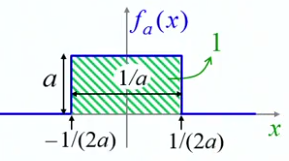
\includegraphics[scale=0.45]{ch1/image1.png}
\captionof{figure}{ }
\end{wrapfigure}
Nous allons commencer par l'étude de la distribution de Dirac, dernier grand 
physicien théoricien du 20$^e$ siècle, notamment en découvrant le positron, 
\dots Ici on va insister sur la \textit{distribution} que l'on peut voir comme 
une généralisation de la notion de fonction. Afin de l'introduire, étudions la 
fonction carrée (ou fenêtre) :


\begin{equation}
f_a(x) =\left\{\begin{array}{ll}
a &\text{ si } |x| \leq \frac{1}{2a}\\
0 &\text{ si } |x| > \frac{1}{2a}
\end{array}\right.
\end{equation}
donnant un carré de hauteur $a$ et de largeur $1/a$, sa surface vaut dès lors 
l'unité. 
\begin{equation}
\int_{-\infty}^\infty f_a(x)\ dx = 1
\label{eq:lim1}
\end{equation}
La distribution de dirac peut etre définie à partir de cette fonction 
en prenant la limite de $a$ tendant vers l'infini : sa hauteur tend vers 
l'infini tandis que sa largeur tend vers zéro.
\begin{equation}
\delta(x) = \lim\limits_{a\rightarrow\infty} f_a(x)
\end{equation}
On va appeler cette distribution $\delta(x)$ qui représente un pic placé en 
zéro, l'origine est le seul point ou l'on trouve une valeur particulière. On 
peut néanmoins dire que la surface sous la courbe vaut l'unité. Cela se 
voit à partir de \autoref{eq:lim1} : la surface sous la courbe ne dépend pas 
du paramètre $a$, d'où la surface unitaire :
\begin{equation}
\int_{-\infty}^\infty \delta(x)\ dx = 1
\end{equation}

\begin{wrapfigure}[7]{l}{4.5cm}
\vspace{-17mm}
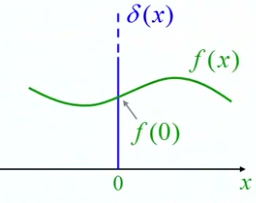
\includegraphics[scale=0.45]{ch1/image2.png}
\captionof{figure}{ }
\end{wrapfigure}
L'intérêt de cette distribution ne se remarque que par combinaison avec d'autres 
fonction. Considérons le produit d'une fonciton quelconque avec la fonction de 
Dirac. La seule fonction qui sera considérée est celle qui se trouve en zéro :
\begin{equation}
f(x)\delta(x) = f(0)\delta(x)
\end{equation}
Toutes les valeurs autres que celle de $x$ n'entre pas en ligne de compte. En 
intégrant ce produit 
\begin{equation}
\int_{-\infty}^{\infty} f(x)\delta(x)\ dx = \int_{-\infty}^\infty f(0)\delta(x)\ dx
= f(0)\int_{-\infty}^{\infty}\delta(x)\ dx = f(0)
\end{equation}
On voit que cette intégrale comme le "produit-scalaire" de $f$ avec $\delta$ qui 
sélectionne la valeur de la fonction à l'origine. En résumé
\begin{equation}
\delta(x) = \left\{\begin{array}{ll}
\infty & \text{ si } x = 0\\
0 & \text{ si } x \neq 0
\end{array} \right.
\end{equation}

\begin{wrapfigure}[7]{l}{4.5cm}
\vspace{-13mm}
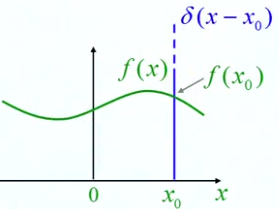
\includegraphics[scale=0.45]{ch1/image3.png}
\captionof{figure}{ }
\end{wrapfigure}
Cette notion peut être généralisée en déplaçant la distribution par translation en 
changeant l'argument $x$ en $x-x_0$ :
\begin{equation}
\delta(x-x_0) = \left\{\begin{array}{ll}
\infty & \text{ si } x=x_0\\
0 & \text{ si } x\neq x_0 
\end{array} \right.
\end{equation}
Cette distribution translatée multipliée par $f$ sélectionnera dès lors $f(x_0)$. 
La distribution de Dirac peut être définie par une infinité de fonction, tendant 
vers cette fameuse distribution lorsque le paramètre $a$ tend vers zéro. On peut 
par exemple prendre la distribution gaussienne 
\begin{equation}
\delta_a(x) = \frac{1}{a\sqrt{\pi}}e^{-x^2/a^2}  
\end{equation}
Lorsque $a$ tend vers zéro, on obtient un \textit{pic} tendant vers l'infini. On 
peut montrer que cette gaussienne, pour cette limite, tend bien vers la distribution 
de Dirac. Dans le cadre de ce cours, consacré à l'optique de Fourier, la distribution 
intéressante est la suivante
\begin{equation}
\delta_a(x) = \frac{1}{\pi x}\sin\left(\frac{x}{a}\right) = \frac{1}{2\pi}\int_{-1/a}^{1/a}
\cos(kx)\ dk
\end{equation}
Il s'agit d'une définition particulière, la suite du cours justifiera pleinement 
l'utilisation de celle-ci (les transformées de Fourier impliquent les fonction 
harmoniques). On va pouvoir trouver la distribution de Dirac à partir de
\begin{equation}
f(\alpha) = \int_{-\infty}^{\infty} \cos(\alpha x)\ dx
\end{equation}
La résultat dépendra de $\alpha$, ce résultat pourrait bien être une fonction de 
$\alpha$ qui se rapprochera très fortement de la distribution recherchée. Par 
intégration
\begin{equation}
f(\alpha) = \int_{-\infty}^{\infty} \cos(\alpha x)\ dx = \frac{1}{\alpha}\left[
\sin(\alpha x)\right]^\infty_{-\infty} = \frac{1}{a}[\sin(\infty)-\sin(-\infty)]
\end{equation}
Nous sommes face ici à une indétermination, cette intégrale généralisée n'est pas 
directement calculable. Il est préférable de travailler avec la fonction d'intégrale 
de Riemann aux bornes réelles pour ensuite faire tendre celle ci vers l'infini
\begin{equation}
\begin{array}{ll}
f(\alpha) = \int_{-L}^L \cos(\alpha x)\ dx &= \frac{1}{\alpha}[\sin(\alpha L)-\sin(-\alpha 
L)]\\
&= \frac{1}{\alpha}[\sin(\alpha L)+\sin(+\alpha L)]\\
&= 2\frac{\sin(\alpha L)}{\alpha}
\end{array}
\end{equation}

\begin{wrapfigure}[8]{r}{4.5cm}
\vspace{-5mm}
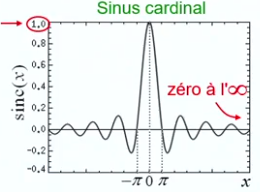
\includegraphics[scale=0.45]{ch1/image4.png}
\captionof{figure}{ }
\end{wrapfigure}
Considérons l'artifice mathématique suivant, permettant de faire apparaître le 
sinus cardinal ($\equiv \sin x/x$) :
\begin{equation}
\begin{array}{ll}
f(\alpha) &= 2L \frac{\sin(\alpha L)}{\alpha L}\\
&= 2L\text{sinc}(\alpha L)
\end{array}
\end{equation}
La fonction sinus cardinal tend vers zéro à l'infini, il s'agit d'une fonction paire dont 
la valeur à l'origine vaut l'unité (valeur donnée par la levée de l'indétermination). Cette 
fonction à des zéros multiples que l'on retrouve à chaque multiple de $\pi$.\newpage

\begin{wrapfigure}[8]{l}{4.5cm}
%\vspace{-5mm}
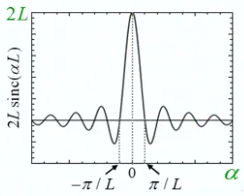
\includegraphics[scale=0.45]{ch1/image5.png}
\captionof{figure}{ }
\end{wrapfigure}
Revenons à nos moutons. Notre fonction sinus cardinal à pour argument $\alpha L$ : les zéros 
de la fonction d'origines se voient tous divisés par $L$ et l'ordonnée à l'origine vaut $2L$. 
Une fois que $\alpha$ n'est plus nul, on redescend brusquement vers un premier zéro (les 
oscillations se comprennent très facilement en interprétant l'aire sous la courbe en faisant 
augmenter $\alpha$).\\
\ \\

\begin{wrapfigure}[8]{r}{7.5cm}
\vspace{-15mm}
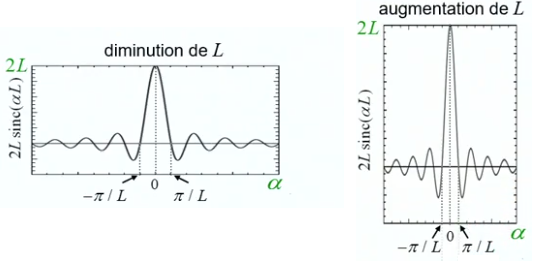
\includegraphics[scale=0.45]{ch1/image6.png}
\captionof{figure}{ }
\end{wrapfigure}
Intéressons nous ce qui se passe lorsque $L \rightarrow \infty$. Remarquons premièrement 
qu'une diminution de $L$ correspond à un \textit{aplatissement} et \textit{élargissent} du 
graphe. Inversement, lorsque $L$ augmente elle gagne en hauteur et les zéros se rapprochent 
de l'origine. Que devient cette fonction pour $L \rightarrow\infty$ ? Montrons que l'on 
obtient, à un facteur près, la distribution de Dirac 
\begin{equation}
f(a) = \lim\limits_{L\rightarrow\infty} \int_{-L}^L \cos(\alpha x)\ dx = \lim\limits_{L 
\rightarrow \infty}[2L\text{sinc}(\alpha L)]
\end{equation}
Cette limite n'est pas facile à appréhender, l'étude du graphe n'est pas fort utile. A 
défaut, on peut s'itnéresser à la surface du graphe de cette fonction en étudiant l'aire 
sous la courbe du sinus cardinal :
\begin{equation}
\int_{-\infty}^\infty \text{sinc }(\alpha x)\ dx = \int_{-\infty}^\infty \dfrac{\sin(\alpha
x)}{\alpha x}\ dx = \dfrac{\pi}{a}
\label{eq:AireD}
\end{equation}
\danger Il ne faut pas confondre la variable $\alpha$ avec celle d'intégration, $x$. Nous 
montrons ici que $f(\alpha)$ peut être associée à la distribution. Dans \autoref{eq:AireD} 
remplaçons $x$ par $\alpha$ par "l'ancien $\alpha$ jouera le rôle du paramètre $L$ :
\begin{equation}
\int_{-\infty}^\infty \text{sinc }(L\alpha)\ d\alpha = \int_{-\infty}^\infty \dfrac{\sin(L\alpha)
}{L\alpha}\ d\alpha = \dfrac{\pi}{L}
\end{equation}
En multipliant par $2L$ (pouvant directement rentrer dans l'intégrale):
\begin{equation}
\int_{-\infty}^\infty2L \text{sinc }(L\alpha)\ d\alpha = \int_{-\infty}^\infty \dfrac{\sin(L\alpha)
}{L \alpha}\ d\alpha = 2\pi
\end{equation}
Cette surface vaut $2\pi$, mais ce qui est important est que celui-ci est indépendant 
du paramètre $L$ exactement comme on l'avait pour la fonction fenêtre avec l'aire unitaire ; 
faire tendre $L$ vers l'infini ne change dès lors rien. Les caractéristiques sont celles de 
la fonction de Dirac. Pour retrouver cette distribution, il nous suffit de diviser par $2\pi$.
\begin{equation}
\int_{-\infty}^\infty \lim\limits_{L\rightarrow\infty}[\frac{2L}{2\pi}\text{sinc}(\alpha L)]\ 
d\alpha = \frac{2\pi}{2\pi}=1
\end{equation}
On peut ainsi assimiler ce résultat à la distribution de Dirac :
\begin{equation}
\text{Distribution de Dirac : } \delta(\alpha) = \lim\limits_{L\rightarrow\infty}\left[
\dfrac{L}{\pi}\text{sinc}(\alpha L)\right]
\end{equation}
Cette fonction est \textit{piquée} à l’origine et une largeur tendant vers zéro dont l'aire
sous la courbe faut bien 1. On peut dès lors écrire
\begin{equation}
f(a) = \lim\limits_{L\rightarrow\infty} \int_{-L}^L \cos(\alpha x)\ dx = \lim\limits_{L 
\rightarrow \infty}[2L\text{sinc}(\alpha L)] = 2\pi \delta(\alpha)
\end{equation}
Sous la forme d'une intégrale généralisée, résultat pratique pour l'étude des transformées 
de Fourier.
\begin{equation}
\int_{-\infty}^\infty \cos(\alpha x)\ dx = 2\pi \delta (\alpha)
\end{equation}
Notons qu'il n'est pas nécessaire de déterminer précisément ce que vaut $\alpha$, la 
"définition" ci-dessous est auto-suffisante
\begin{equation}
\int_{-\infty}^\infty f(\alpha)\delta(\alpha)\ d\alpha = f(0)
\end{equation}
Généralisons quelque peu ce que nous venons de faire en vue de passer à la transformée de 
Fourier. La notion de phaseur, exponentielle imaginaire est fondamentale :
\begin{equation}
\int_{-\infty}^\infty e^{i\alpha x}\ dx = \int_{-\infty}^\infty \cos(\alpha x)\ dx + i
\int_{-\infty}^\infty \sin(\alpha x)\ dx
\end{equation}
Cette exponentielle imaginaire cache la fonction $cos(\alpha x)$ que nous venons d'étudier 
avec en plus une partie imaginaire. Que vaut la contribution de la partie imaginaire ? 
\begin{equation}
\int_{-L}^L \sin(\alpha x)\ dx = -\frac{1}{\alpha}\left[\cos(\alpha x)\right]^L_{-L} = 0
\end{equation}
Il n'est même pas ici nécessaire de faire tendre $L\rightarrow\infty$, le cosinus étant 
une fonction paire cela donne tout simplement zéro (directement visible, car l'intégration 
d'une fonction impaire aux bornes centrées sur zéro est identiquement nulle). \\
En conclusion:
\begin{equation}
\dfrac{1}{2\pi}\int_{-\infty}^\infty e^{i\alpha x}\ dx  = \delta(\alpha)
\end{equation}

\newpage
\section{Transformée de Fourier : introduction}
La transformée de Fourier s'applique à une fonction $f(x)$. Pour transformer celle-ci, il 
faut préalablement mutliplier par $e^{i\alpha x}$ puis intégration :
\begin{equation}
TF(f) \equiv \int_{-\infty}^\infty f(x)e^{i\alpha x}\ dx = F(\alpha)
\end{equation}
où $F(\alpha)$ est la transformée de Fourier de $f(x)$. Le résultat est bien une fonction 
du paramètre $\alpha$ ! Afin d'illustrer cette définition, reconsidérons le premier exemple 
du chapitre, la fonction fenêtre, cette fois-ci non normalisée.
\begin{equation}
f_a(x) =\left\{\begin{array}{ll}
a &\text{ si } |x| \leq L\\
0 &\text{ si } |x| > L
\end{array}\right.
\end{equation}
Calculons sa transformée de Fourier
\begin{equation}
\begin{array}{ll}
TF(f) &= \int_{-L}^L ae^{i\alpha x}\ dx = a\left[\dfrac{1}{i\alpha}e^{i\alpha x}\right]^L_{-L}\\
&= a\dfrac{1}{1\alpha}\left[e^{i\alpha L}-e^{-i\alpha L}\right] = 2a\dfrac{\sin(\alpha L)}{\alpha}
\end{array}
\end{equation}

\begin{wrapfigure}[8]{l}{4.5cm}
\vspace{-25mm}
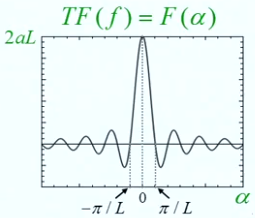
\includegraphics[scale=0.45]{ch1/image7.png}
\captionof{figure}{ }
\end{wrapfigure}
On reconnaît ce que l'on trouvait pour la fonction de Dirac. En multipliant par $L/L$, on obtient 
la transformée de Fourier de la fonction fenêtre
\begin{equation}
TF(f) = 2aL\text{sinc}(\alpha L)
\end{equation}
Il n'y a pour l'instant pas grand chose à comprendre, il ne s'agit que de l'application d'une 
définition. Quel est l'intérêt mathématique de cette transformation? Cette transformation est-elle
réversible ? Oui, c'est son intérêt majeur: la transformée de Fourier inverse.\\
Pour y arriver, étudions la fonction suivante
\begin{equation}
\int_{-\infty}^\infty F(\alpha)e^{-i\alpha x}\ d\alpha  = g(x)
\end{equation}
\danger Il s'agit bien d'un moins, d'où le \textit{inverse}. Le but est de calculer cette intégrale 
pour déterminer notre fameuse inverse dont le résultat sera une fonction de $x$. Remplaçons $F(\alpha)$ 
par son expression (on note $x'$ pour ne pas confondre les variables)
\begin{equation}
g(x)= \int_{-\infty}^\infty \int_{-\infty}^\infty  f(x')e^{i\alpha x'}\ dx'\ e^{-i\alpha x}\ d\alpha
\end{equation}
Par Fubini
\begin{equation}
\begin{array}{ll}
g(x) &= \int_{-\infty}^\infty  f(x') \int_{-\infty}^\infty  e^{i\alpha x'}e^{-i\alpha x}\ d\alpha\ dx'\\
&= \int_{-\infty}^\infty  f(x') \int_{-\infty}^\infty  e^{i\alpha (x'-x)}\ d\alpha\ dx'
\end{array}
\end{equation}
En utilisant une des définition de la distribution de Dirac : $\dfrac{1}{2\pi}\int_{-\infty}^\infty 
e^{i\alpha x}\ dx  = \delta(\alpha)$ en remplaçant $\alpha$ par $x$ et l'ancien $\alpha$ par $L$ :
\begin{equation}
g(x) = \int_{-\infty}^\infty  f(x')\ 2\pi\delta(x'-x)\ dx' = 2\pi f(x)
\end{equation}
Cette intégrale ne sélectionne que la valeur de la fonction $f$ lorsque $x=x'$. 
\begin{equation}
g(x) = \int_{-\infty}^\infty F(\alpha)e^{-i\alpha x}\ d\alpha  = g(x) = 2\pi f(x)
\end{equation}
La \textbf{transformée de Fourier inverse} est donne par
\begin{equation}
TF^{-1}(F) = \frac{1}{2\pi}\int_{-\infty}^\infty F(\alpha)e^{-i\alpha x}\ d\alpha = f(x)
\end{equation}
Petite relation intéressante :
\begin{equation}
TF^{-1}[TF(f)] = f(x)
\end{equation}

\begin{wrapfigure}[6]{l}{5.5cm}
\vspace{-10mm}
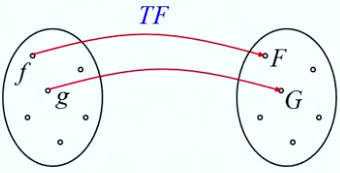
\includegraphics[scale=0.45]{ch1/image8.png}
\captionof{figure}{ }
\end{wrapfigure}
Ceci montre que la transformée de Fourier est une bijection dans l'espace des fonctions. A 
quelques restrictions près, on peut transformer toutes les fonctions par Fourier. Il s'agit 
d'une bijection car deux fonctions distinctes donneront deux transformées différentes, ceci 
vient de l'existence de la transformée inverse. 
\begin{proof}\ \\
\begin{equation}
\begin{array}{ll}
TF(f) = F &\Longrightarrow TF^{-1}[TF(f)] = TF^{-1}[F] = f\\
TF(g) = F &\Longrightarrow TF^{-1}[TF(g)] = TF^{-1}[F] = f = g
\end{array}
\end{equation}
\end{proof}
Il sera dès lors toujours possible de "défaire" une transformée de Fourier de façon univoque. 
Illustrons à nouveau, cette fois-ci avec une gaussienne :
\begin{equation}
f(x) = e^{-x^2/x_0^2}\quad \ft \quad F(\alpha) = x_0\sqrt{\pi}e^{-\alpha^2x_0^2/4}
\end{equation}
Résultat un peu plus compliqué à trouver, il est nécessaire d'utiliser l’analyse complexe. On 
remarque que le résultat est également une gaussienne dont la largeur est inversement 
proportionnelle à $x_0$. Plus la gaussienne est étroite, plus $x_0$ est petit, plus la transformée 
inverse sera large\footnote{Aussi valable pour la fonction fenêtre.}.
Plus la fonction est large, plus sa transformée est étroite et vice-versa la règle est vraiment 
très générale.
\begin{center}
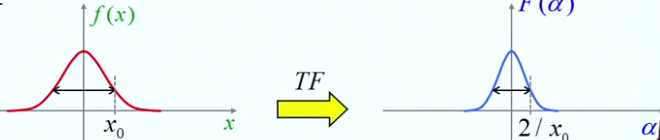
\includegraphics[scale=0.45]{ch1/image9.png}
\captionof{figure}{ }
\end{center}

En faisant tendre $x_0 \rightarrow$ et en supposant une normalisation, on retrouve le delta de 
Dirac $f(x) = \delta(x)$. On peut montrer que si on fait ça, la gaussienne dans le domaine de 
Fourier tend vers l'infini : c'est une constante. Pour trouver la valeur de celle-ci, calculons
\begin{equation}
F(\alpha) = \int_{-\infty}^\infty \delta(x) e^{i\alpha x}\ dx = 1
\end{equation}\\

Considérons un autre exemple : $f(x) = e^{-i\alpha_0x}$. Par application de la définition
\begin{equation}
F(\alpha) = \int_{-\infty}^\infty e^{i(\alpha-\alpha_0)}\ dx = 2\pi\delta(\alpha-\alpha_0)
\end{equation}
\begin{center}
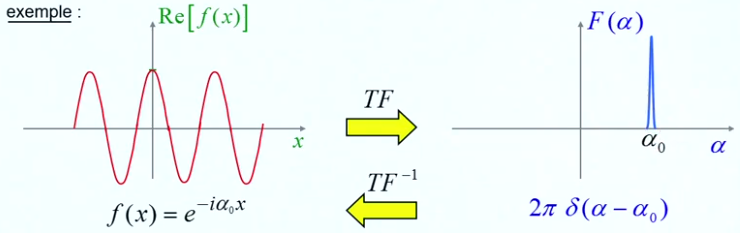
\includegraphics[scale=0.45]{ch1/image10.png}
\captionof{figure}{ }
\end{center}
Le $\alpha_0$ imposant la périodicité de la fonction harmonique localise le "pic" du delta 
de Dirac. La transformée de Fourier de l'exponentielle imaginaire donne directement le delta 
de Dirac. Plutôt que de prendre l'exponentielle je peux faire de même avec le cosinus directement :
\begin{equation}
f(x) = \cos(\alpha_0x) = \frac{e^{i\alpha_0x}+e^{-i\alpha_0x}}{2}
\end{equation}
La seule différence est la contribution de la partie imaginaire
\begin{equation}
F(\alpha) = \int_{-\infty}^\infty f(x)e^{i\alpha x}\ dx = \pi[\delta(\alpha+\alpha_0)+\delta(\alpha
-\alpha_0)]
\end{equation}
\begin{center}
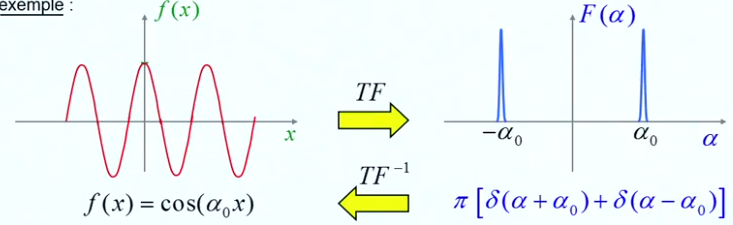
\includegraphics[scale=0.45]{ch1/image11.png}
\captionof{figure}{ }
\end{center}
Dans le cas d'un sinus, il faudra mettre un signe négatif entre les delta et diviser par $i$.\\

Passons en revues les propriétés des transformées de Fourier. Soit la transformée de Fourier
\begin{equation}
F(\alpha) = \int_{-\infty}^\infty f(x)e^{i\alpha x}\ dx
\end{equation}
\begin{equation}
\begin{array}{lll}
\bullet & TF[f(x-x_0)] &= \int_{-\infty}^\infty f(x-x_0)e^{i\alpha x}\ dx\\
&&= \int_{-\infty}^\infty f(x')e^{i\alpha (x'+x_0)}\ dx'\\
&&= e^{i\alpha x_0}\int_{-\infty}^\infty f(x')\ dx'\\
&&= F(\alpha)e^{i\alpha x_0}\ \\
\ \\
\bullet & TF^{-1}[F(\alpha-\alpha_0)] &= f(x)e^{-i\alpha_0 x}\\
\bullet & TF[f(x)e^{-i\alpha_0x}] &= F(\alpha-\alpha_0)
\end{array}
\end{equation}
Ceci peut se résumer avec la fonction de Dirac
\begin{equation}
TF[\delta(x-x_0)] = e^{i\alpha x_0},\qquad TF[e^{-i\alpha_0x}] = \delta(\alpha-\alpha_0)
\end{equation}
Intéressons-nous maintenant à la transformée de Fourier de la dérivée de $f(x)$. Le plus 
simple est d'utiliser la notion de transformée de Fourier inverse
\begin{equation}
f(x) = \frac{1}{2\pi}\int_{-\infty}^\infty F(\alpha)e^{-i\alpha x}\ d\alpha
\end{equation}
En dérivant
\begin{equation}
\begin{array}{ll}
\dfrac{df(x)}{dx} &= \frac{1}{2\pi}\int_{-\infty}^\infty -i\alpha F(\alpha)e^{-i\alpha x}\ 
d\alpha\\
&= TF^{-1}[-i\alpha F(\alpha)]
\end{array}
\end{equation}
On a donc
\begin{equation}
TF\left[\dfrac{df(x)}{dx}\right] = -i\alpha F(\alpha)
\end{equation}
Pour une dérivée seconde, on trouvera $(-i\alpha)^2$, \dots\\

Terminons la section par une généralisation de la transformée de Fourier à deux dimensions. 
Considérons une fonction à deux variables que l'on va multiplier par deux exponentielles de 
sorte à avoir deux variables de Fourier (dites conjuguées, l'une à $x$, l'autre à $y$):
\begin{equation}
F(\alpha,\beta) = \int_{-\infty}^\infty\int_{-\infty}^\infty f(x,y)e^{i\alpha x}e^{i\beta y}\ 
dx\ dy
\end{equation}
A condition de montrer que $f(x,y)$ peut être écrite à partir de la transformée de Fourier 
inverse, on obtient la transformée de Fourier inverse à deux dimensions
\begin{equation}
f(x,y) = \frac{1}{(2\pi)^2} \int_{-\infty}^\infty\int_{-\infty}^\infty F(\alpha,\beta)
e^{-i\alpha x}e^{-i\beta y}\ d\alpha\ d\beta
\end{equation}
Ceci est cohérent et pour s'en rendre compte, substituons l'expression de $F(\alpha,\beta)$ :
\begin{equation}
f(x,y) = \frac{1}{(2\pi)^2} \int_{-\infty}^\infty\int_{-\infty}^\infty \int_{-\infty}^\infty
\int_{-\infty}^\infty f(x',y')e^{i\alpha x'}e^{i\beta y'}\ e^{-i\alpha x}e^{-i\beta y}\
 d\alpha\ d\beta\ dx'\ dy' 
\end{equation}
Par Fubini
\begin{equation}
f(x,y) = \frac{1}{(2\pi)^2} \int_{-\infty}^\infty\int_{-\infty}^\infty f(x',y') \int_{-\infty}^\infty
\int_{-\infty}^\infty e^{i\alpha x'}e^{i\beta y'}\ e^{-i\alpha x}e^{-i\beta y}\
 d\alpha\ d\beta\ dx'\ dy' 
\end{equation}
En intégrant sur $\alpha$
\begin{equation}
f(x,y) = \frac{1}{(2\pi)^2} \int_{-\infty}^\infty\int_{-\infty}^\infty f(x',y') \underbrace{
\int_{-\infty}^\infty e^{i\alpha(x'-x)}\ d\alpha}_{2\pi\delta(x'-x)} \underbrace{\int_{-\infty}^\infty 
e^{i\beta(y'-y)}\ d\beta}_{2\pi\delta(y'-y)}\ dx'\ dy'
\end{equation}
On voit apparaître la distribution de Dirac, de sorte à pouvoir écrire
\begin{equation}
f(x,y) = \int_{-\infty}^\infty\int_{-\infty}^\infty f(x',y')\delta(x'-x)\delta(y'-y)\ dx'\ dy'
\end{equation}
En appliquant la notion de Distribution de Dirac qui "sélectionne" l'argument de la fonction tel 
que l'argument de la fonction de Dirac s'annule c'est à dire que $x'=x$ et $y'=y$. Ce résultat-ci 
est bien $f(x,y)$, pas besoin d'aller plus loin. Ceci prouve que le résultat est cohérent.





\newpage
\section{Transformée de Fourier : convolution}

























